\documentclass{article}


\usepackage{arxiv}

\usepackage[utf8]{inputenc} % allow utf-8 input
\usepackage[T1]{fontenc}    % use 8-bit T1 fonts
\usepackage{hyperref}       % hyperlinks
\usepackage{url}            % simple URL typesetting
\usepackage{booktabs}       % professional-quality tables
\usepackage{amsfonts}       % blackboard math symbols
\usepackage{nicefrac}       % compact symbols for 1/2, etc.
\usepackage{microtype}      % microtypography
\usepackage{lipsum}
\usepackage{graphicx,wrapfig}
\usepackage{caption}

\title{A template for the \emph{arxiv} style}


\author{
  David Unger\thanks{Use footnote for providing further
    information about author (webpage, alternative
    address)---\emph{not} for acknowledging funding agencies.} \\
  Department of Computer Science\\
  Cranberry-Lemon University\\
  Pittsburgh, PA 15213 \\
  \texttt{hippo@cs.cranberry-lemon.edu} \\
  %% examples of more authors
   \And
  Nick Wagner\\
  3524444 \\
  M.Sc. Autonome Systeme\\
  University of Stuttgart\\
  \texttt{st175644@stud.uni-stuttgart.de} \\
  %% \AND
  %% Coauthor \\
  %% Affiliation \\
  %% Address \\
  %% \texttt{email} \\
  %% \And
  %% Coauthor \\
  %% Affiliation \\
  %% Address \\
  %% \texttt{email} \\
  %% \And
  %% Coauthor \\
  %% Affiliation \\
  %% Address \\
  %% \texttt{email} \\
}

\begin{document}
\maketitle

\begin{abstract}
Diabetic retinopathy is an eye disease that can affect people suffering diabetes. It causes damage to the blood vessels of 
the eyes, deteriorates the eyesight and can lead in the worst case to blindness of the patient. It is important to 
detect the disease in an early stage to mitigate it as good as possible with an early treatment. Analyzing images of 
eyes and classify the severity of diabetic retinopathy is a challenging task that requires expert knowledge. To assist 
doctors and medical personnel, a classification model shall be trained to classify the severity automatically. 
\end{abstract}

% 1 %%%%%%%%%%%%%%%%%%%%%%%%%%%%%%%%%%%%%%%%%%%%%%%%%%%%%%%%%%%%%%%%%%%%%%%%%%%%%%%%%%%%%%%%%%%%%%%%%%%%%%%%%%%%%%%%%%%%%%
\section{Introduction}
Diabetic retinopathy is a complication of diabetes, which can cause damage the retina of the eye. 
If not detected early, this damage may cause cause vision impairment or even blindness. 
To treat this condition successfully, it has to be detected at an early stage, which is difficult due to minimal to no early warning signs. 
Furthermore, the different grades can only be distinguished by a trained professional due to its subtle symptoms.
Examples are leaking blood vessels, fatty deposits or retinal swelling.
Since this task is difficult even for trained professionals, an algorithm for automatic detection of the diabetic retinopathy grade is necessary.
This is the goal of this paper. 


Dataset
% 2 %%%%%%%%%%%%%%%%%%%%%%%%%%%%%%%%%%%%%%%%%%%%%%%%%%%%%%%%%%%%%%%%%%%%%%%%%%%%%%%%%%%%%%%%%%%%%%%%%%%%%%%%%%%%%%%%%%%%%%
\section{Object Classification}
\subsection{Problem analysis}

To tackle the problem of diabetic retinopathy detection, several methods are possible. Because the dataset consists of 
ordinally scaled data of 5 classes, regression could be used to estimate the serverity of a case. In addition, a the problem 
can be handled as a classification problem after one-hot-encoding the labels. As a third option, one can define a threshold 
to define problematic diabetic retinopathy and non-problematic diabetic retinopathy and can handle the problem as a binary 
classification. Further, only binary and multiclass classification are anaylzed.

A binary classification has the advantage of higher accuracy, but lacks details, because the network only outputs 0 or 1
and no information about the exact serverity of the disease. Metrics are also easy to implement, because precision, 
recall and f1-score are standard implementations and nicely interpretable.

A multiclass classification has typically a lower accuracy, because the network needs to pick the right class among 
several classes. It provides the benefit or receiving richer information, i.e. the exact serverity of the disease.
Evaluating a multiclass classification problem becomes harder, because missclassifications can vary in their error.
Classifiying a class 1 as class 2 is for example less problematic than classifying class 1 as class 5.


\subsection{Architecture}
VGG, Resnet, Weight freeeze / unfreeze, GAP, Flatten, Dense Layers
\subsection{Weight initialization}
Weight initialization refers to the initial values of parameters that are used in specific neural network layers.
Changing the initialization of the layers changes the starting point for the optimization process and potentially also the performance.
Keras initializes the weights of dense layers with the Glorot uniform initializer, which draws samples from a truncated uniform distribution.
Generally the goal is to avoid vanishing and exploding gradients, even better is if the variance of layer outputs is approximately one. [paper KUMAR]
Specifically for the ReLU activation function, this is achieved with the He initialization, which draws from a normal distribution with the following parameters. [paper HE]\\
\begin{minipage}{.5\linewidth}
  \begin{equation}
    \mu = 0
  \end{equation}
\end{minipage}
\begin{minipage}{.5\linewidth}
  \begin{equation}
    \sigma^2 = 2/N
  \end{equation}
\end{minipage}

This led to a faster training and performance increase of X percent.

\subsection{Augmentation}
Within the input pipeline three main types of augmentation are applied.
The goal is to make feature extraction easier for the network and increase the amount of input images which reduces overfitting.
\begin{itemize}
  \item[-] \textbf{Graham preprocessing:} \begin{itemize}
    \item[1.] rescale the eye radius to 300 pixels 
    \item[2.] subtract the local average color such that the local average gets mapped to gray
    \item[3.] clip the image to remove boundary effects
    \begin{figure}[h]
      \begin{minipage}[b]{.5\textwidth}
          \begin{center}
          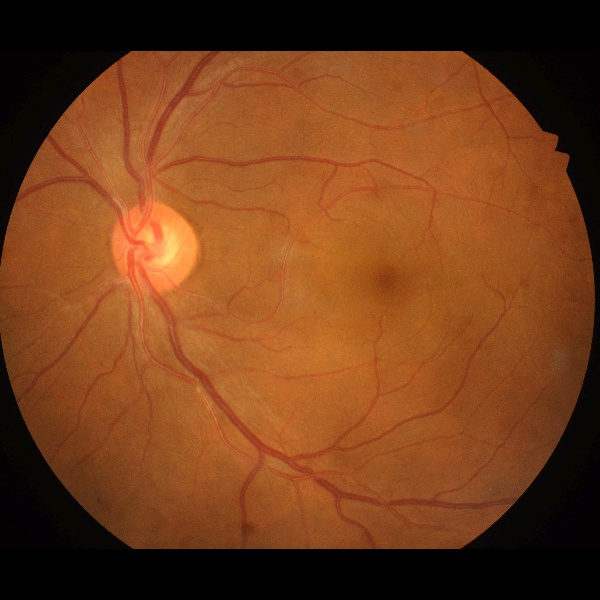
\includegraphics[width=.5\linewidth]{IDRiD_060.jpg}
          \captionsetup{justification=centering}
          \captionof{figure}{original image}
          \label{fig:IDRiD}
          \end{center}
      \end{minipage}%
      \begin{minipage}[b]{.5\textwidth}
          \begin{center}
          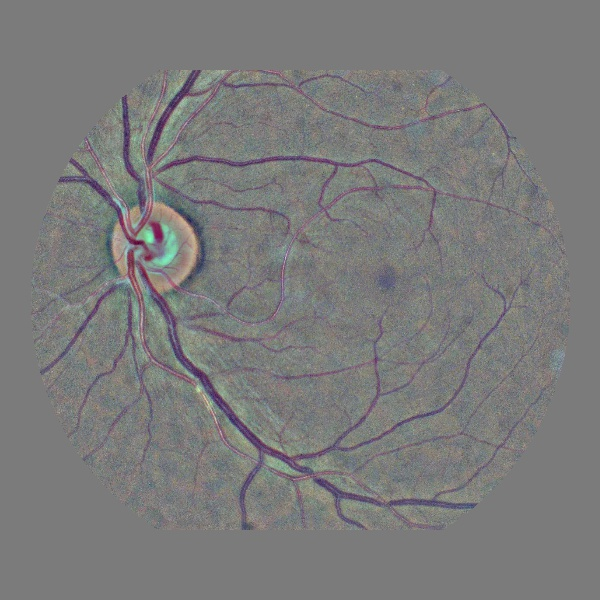
\includegraphics[width=.5\linewidth]{IDRiD_060_graham.jpg}
          \captionsetup{justification=centering}
          \captionof{figure}{graham preprocessed image}
          \label{fig:IDRiD_graham}
          \end{center}
      \end{minipage}
  \end{figure} 
  \end{itemize}   
  \item[-] \textbf{Color jittering:} Slight random changes to brightness, hue, saturation or contrast.
  \item[-] \textbf{Random cropping:} Crop a window that is slightly smaller than the image. Then resize to original size again.
\end{itemize}
\subsection{Dataset Balancing}
Two types of dataset balancing were evaluated. First class-balancing and second oversampling.
\subsection{Training}
Adam, SGD, Momentum, Learing rate decay
\subsection{Metrics}
incl. QWC
% 3 %%%%%%%%%%%%%%%%%%%%%%%%%%%%%%%%%%%%%%%%%%%%%%%%%%%%%%%%%%%%%%%%%%%%%%%%%%%%%%%%%%%%%%%%%%%%%%%%%%%%%%%%%%%%%%%%%%%%%%
\section{Experiments}
\subsection{Procedure}
The training of the deep neural network classifier requires the selection of suitable hyperparameters that differ from
problem to problem. A useful strategy to find a good set of hyperparameters are parameter sweeps. Weights\&Biases is a 
python library that enables the easy implementation of sweeps. 

Hyperparameter optimization requires besides training and test dataset a third, the validation dataset, to evaluate the
model after hyperparameter tuning and to avoid overfitting on the hyperparameters. Because the given dataset only contains 
training and test data, the original training dataset was split into 80\% training data and 20\% validation data.

In total, x sweeps consisting of x runs and x epochs were performed during the project.

\subsection{Hyperparameter selection}
The following parameters show a big effect on the performance of the neural network on the validation data, 
why they are selected for the final classifier.

Balancing

...

\subsection{Grad cam}
% 4 %%%%%%%%%%%%%%%%%%%%%%%%%%%%%%%%%%%%%%%%%%%%%%%%%%%%%%%%%%%%%%%%%%%%%%%%%%%%%%%%%%%%%%%%%%%%%%%%%%%%%%%%%%%%%%%%%%%%%%
\section{Results}
best binary + multiclass performance;
color coded confusion matrix

%%%%%%%%%%%%%%%%%%%%%%%%%%%%%%%%%%%%%%%%%%%%%%%%%%%%%%%%%%%%%%%%%%%%%%%%%%%%%%%%%%%%%%%%%%%%%%%%%%%%%%%%
%%%%%%%%%%%%%%%%%%%%%%%%%%%%%%%%%%%%%%%%%%%%%%%%%%%%%%%%%%%%%%%%%%%%%%%%%%%%%%%%%%%%%%%%%%%%%%%%%%%%%%%%
%%%%%%%%%%%%%%%%%%%%%%%%%%%%%%%%%%%%%%%%%%%%%%%%%%%%%%%%%%%%%%%%%%%%%%%%%%%%%%%%%%%%%%%%%%%%%%%%%%%%%%%%
% below is just there for some help with the formatting
\section{Headings: first level}
\label{sec:headings}

\lipsum[4] See Section \ref{sec:headings}.

\subsection{Headings: second level}
\lipsum[5]
\begin{equation}
\xi _{ij}(t)=P(x_{t}=i,x_{t+1}=j|y,v,w;\theta)= {\frac {\alpha _{i}(t)a^{w_t}_{ij}\beta _{j}(t+1)b^{v_{t+1}}_{j}(y_{t+1})}{\sum _{i=1}^{N} \sum _{j=1}^{N} \alpha _{i}(t)a^{w_t}_{ij}\beta _{j}(t+1)b^{v_{t+1}}_{j}(y_{t+1})}}
\end{equation}

\subsubsection{Headings: third level}
\lipsum[6]

\paragraph{Paragraph}
\lipsum[7]

\section{Examples of citations, figures, tables, references}
\label{sec:others}
\lipsum[8] \cite{kour2014real,kour2014fast} and see \cite{hadash2018estimate}.

The documentation for \verb+natbib+ may be found at
\begin{center}
  \url{http://mirrors.ctan.org/macros/latex/contrib/natbib/natnotes.pdf}
\end{center}
Of note is the command \verb+\citet+, which produces citations
appropriate for use in inline text.  For example,
\begin{verbatim}
   \citet{hasselmo} investigated\dots
\end{verbatim}
produces
\begin{quote}
  Hasselmo, et al.\ (1995) investigated\dots
\end{quote}

\begin{center}
  \url{https://www.ctan.org/pkg/booktabs}
\end{center}


\subsection{Figures}
\lipsum[10] 
See Figure \ref{fig:fig1}. Here is how you add footnotes. \footnote{Sample of the first footnote.}
\lipsum[11] 

\begin{figure}
  \centering
  \fbox{\rule[-.5cm]{4cm}{4cm} \rule[-.5cm]{4cm}{0cm}}
  \caption{Sample figure caption.}
  \label{fig:fig1}
\end{figure}

\subsection{Tables}
\lipsum[12]
See awesome Table~\ref{tab:table}.

\begin{table}
 \caption{Sample table title}
  \centering
  \begin{tabular}{lll}
    \toprule
    \multicolumn{2}{c}{Part}                   \\
    \cmidrule(r){1-2}
    Name     & Description     & Size ($\mu$m) \\
    \midrule
    Dendrite & Input terminal  & $\sim$100     \\
    Axon     & Output terminal & $\sim$10      \\
    Soma     & Cell body       & up to $10^6$  \\
    \bottomrule
  \end{tabular}
  \label{tab:table}
\end{table}

\subsection{Lists}
\begin{itemize}
\item Lorem ipsum dolor sit amet
\item consectetur adipiscing elit. 
\item Aliquam dignissim blandit est, in dictum tortor gravida eget. In ac rutrum magna.
\end{itemize}


\bibliographystyle{unsrt}  
%\bibliography{references}  %%% Remove comment to use the external .bib file (using bibtex).
%%% and comment out the ``thebibliography'' section.


%%% Comment out this section when you \bibliography{references} is enabled.
\begin{thebibliography}{1}

\bibitem{kumar2017weight}
Siddharth Krishna Kumar.
\newblock On weight initialization in deep neural networks.
\newblock {\em arXiv:1704.08863}, 2017.

\bibitem{kumar2017weight}
name.
\newblock title.
\newblock In {\em Frontiers in Handwriting Recognition (ICFHR), 2014 14th
  International Conference on}, pages 417--422. IEEE, 2014.

\end{thebibliography}

\end{document}
